%---Hyperref settings---------------------------------------------------------%

\documentclass[11pt,a4paper]{report}

\usepackage{fullpage}                  % Use full page
\usepackage[usegeometry]{typearea}     % before geometry!
\usepackage{geometry}
\geometry{
a4paper,
left=20mm,
right=20mm,
top=13mm,
bottom=25mm,
headsep=10mm,
headheight=-10mm,
footskip=22mm,
includefoot
}
\usepackage[french]{babel}             % Set language
\usepackage{cmbright}
\usepackage[T1]{fontenc}               % Needed when using french
\usepackage[utf8]{inputenc}            % Set to UTF-8
\usepackage{csquotes}                  % To quote some text
\usepackage{pdfpages}                  % To set PDF styles
\usepackage{hyperref}                  % To create hyperlinks in cross references
\usepackage{graphicx}                  % To insert images
\usepackage{color}                     % To create colored text and background
\usepackage{float}                     % To change image floating
\usepackage{url}                       % To refer to URLs
\usepackage{caption}                   % To add caption to tables
\usepackage{etoolbox}
\usepackage{titlesec}
\usepackage{lscape}
\usepackage{pdfpages}
\usepackage{pdflscape}
\usepackage{parskip}


%---Chapter and other settings------------------------------------------------%
\setcounter{secnumdepth}{4}
\setcounter{tocdepth}{4}

\titleformat{\chapter}{\normalfont\huge}{\textbf\thechapter}{20pt}{\huge\textbf}
\titlespacing*{\chapter}{0pt}{0pt}{20pt}

\makeatletter
\patchcmd{\chapter}{\if@openright\cleardoublepage\else\clearpage\fi}{}{}{}
\makeatother

\newcommand*{\useportrait}{%
  \clearpage
  \KOMAoptions{paper=portrait,DIV=current}%switch to portrait
    \newgeometry{% geometry settings for portrait
    left=2cm, right=2cm, top=2cm, bottom=2cm, headsep=1mm,
    }%
  \fancyhfoffset{0pt}% <- recalculate head and foot width for fancyhdr
}
\newcommand*{\uselandscape}{%
  \clearpage
  \KOMAoptions{paper=landscape,DIV=current}%switch to landscape
    \newgeometry{% geometry settings for portrait
        left=2cm, right=2cm, top=3cm, bottom=0.5cm, includefoot
    }%
  \fancyhfoffset{0pt}% recalculate head and foot width for fancyhdr
}


\definecolor{mygreen}{rgb}{0.80784, 0.89412, 0.59608}


%---Maketitle metadata--------------------------------------------------------%

\newcommand{\horrule}[1]{\rule{\linewidth}{#1}} 	% Horizontal rule

%---Custom commands-----------------------------------------------------------%

\newcommand*{\fullref}[1]{\hyperref[{#1}]{\autoref*{#1} \nameref*{#1}}}

%---Custom headers/footers (fancyhdr package)---------------------------------%

\usepackage{fancyhdr}
\pagestyle{fancyplain}
\fancyhead[L]{\setlength{\unitlength}{1mm}
\begin{picture}(0,0)
\put(-7,-4.5){
\includegraphics[width=5cm]{rsc/mse_logo.png}}
\end{picture}}
\fancyhead[C]{Rapport - Projet - WEM}
\fancyhead[R]{\setlength{\unitlength}{1mm}
\begin{picture}(0,0)
\put(-29,-3.5){
\includegraphics[width=3cm]{rsc/hes_logo.png}}
\end{picture}}
\fancyfoot[C]{\begin{picture}(0,0)
        \put(0,30){\thepage}
\end{picture}}
\renewcommand{\headrulewidth}{0pt}
\renewcommand{\footrulewidth}{0pt}
\setlength{\headheight}{13.6pt}

\begin{document}

%---Hyperref settings---------------------------------------------------------%

\hypersetup{pdfauthor={Andrea Petrucci, Benjamin Pasquier, Laurent Hirschi},
            pdftitle=Cahier des charges - Web Mining - Wine Recommender,
            pdfsubject=IT}

%---Title---------------------------------------------------------------------%

\title{
        
\includegraphics[width=10cm]{rsc/mse_logo.png} \\
        
        \horrule{2pt} \\[0.4cm]
        \huge{\textbf{Cahier des charges - WEM - Wine Recommender}}\\
        \horrule{1pt} \\[0.5cm]
        Master MSE
        \horrule{2pt} \\[0.5cm]
        }
\author{Rédigé par: \textbf{Andrea Petrucci, Benjamin Pasquier, Laurent Hirschi} \vspace{2mm} \\
                    \textbf{Groupe D} \vspace{5mm} \\
        Supervisé par: Dr. Laura Elena Raileanu \vspace{2mm} \\
        Assistants: Elena Najdenovska et Cédric Campos Carvalho \vspace{5mm} \\
        Version: 1.0}
\date{\today}
\maketitle

%---Versions table------------------------------------------------------------%

\chapter*{Table des versions}
\pagenumbering{gobble}
        \begin{table}[H]
        \begin{tabular}{|p{2cm}|p{14.1cm}|}
        \hline
        \textbf{Version} & \textbf{Description} \\ \hline
        1.0 & Version initiale \\  \hline  
        \end{tabular}
\end{table}

%---Contents------------------------------------------------------------------%

\addtocontents{toc}{\protect
\pagenumbering{gobble}}
\tableofcontents
\newpage

%---Figures-------------------------------------------------------------------%

\addtocontents{toc}{\protect
\pagenumbering{gobble}}
\listoffigures
\newpage

%---Chapters------------------------------------------------------------------%

\chapter{Contexte et objectifs}
\pagenumbering{arabic}
Dans le cadre du cours de Web Mining, il est demandé de réaliser un projet de récupération et d'analyse de données.
Le sujet choisi pour ce dernier est la création d'un système de recommandation de vin en fonction d'une recette.


\section{Contexte}
Lorsque nous choisissons de préparer une recette, nous nous demandons parfois quel vin accompagnerait le mieux ce plat. 
En règle générale, les descriptifs de vins viennent accompagnés d'une recommandation du style "boeuf", "poulet", "poisson", etc.
Mais ces recommandations sont souvent trop générales et ne permettent pas de choisir un vin adapté à la recette. 
De plus, il est difficile de trouver des informations sur les vins, notamment sur les vins de qualité moyenne ou inférieure. 
C'est pourquoi nous avons décidé de créer un système de recommandation de vin en fonction d'une recette sous forme d'une application web.

Pour ce faire, deux sources de données seront utilisées:
\begin{itemize}
    \item \href{https://www.vivino.com/}{\textbf{Vivino}}: pour la récupération des données sur les vins.
    \item \href{https://www.marmiton.org/recettes/index/categorie/plat-principal/}{\textbf{Marmiton}}: pour la récupération des données sur les recettes.
\end{itemize}

Afin de traiter une quantité de données raisonnable, nous nous limitons aux plats principaux pour les recettes et aux vins rouges et blancs pour les vins.

\section{Objectifs}
La réalisation du projet est composé de trois parties principales:
\begin{itemize}
    \item \textbf{Récupération des données}: récupération des données sur les vins et les recettes.
    \item \textbf{Création de l'API}: création d'une API REST pour servir les données.
    \item \textbf{Création de l'application web}: création d'une application web pour la recommandation de vin.
\end{itemize}
\newpage

\chapter{Données}
Ce chapitre décrit les données que nous utiliserons dans ce projet et la façon dont elles seront extraites.

\section{Sources des données}

Deux sources de données sont considérés pour la réalisation du projet: le site web Vivino qui répertorie des vins et le site web Marmiton qui répertorie des recettes.

\subsection{Vivino}
Vivino est un site web et une application mobile qui permet de trouver des informations sur une grande quantité de vins.
C'est une plateforme communautaire qui permet aux utilisateurs de donner leur avis sur les vins qu'ils ont dégustés,
d'en trouver des similaires à ceux qu'ils ont appréciés ou en fonction de leur budget.
Le site permet de filtrer les vins en fonction de leur couleur, de leur pays d'origine, de leur région, de leur cépage, etc.
Pour notre projet, nous avons décidé de nous limiter aux vins rouges et blancs provenant de Suisse, d'Argentine, des États-Unis,
de France, d'Italie et d'Espagne, afin de ne pas avoir une quantité trop importante de données à traiter.

\subsection{Marmiton}
Marmiton est un site web qui permet de trouver des recettes de cuisine.
On peut y trouver des recettes de tous types de plats, de l'entrée au dessert.
Notre projet se concentrant sur les plats principaux, nous avons décidé de nous limiter à cette catégorie.

\section{Description des données}

Les deux sources de données considérées contiennent une certaine quantité d'informations dont certaines ne sont pas pertinentes pour notre projet. Il est donc nécessaire de sélectionner les attributs qui nous seront utiles.

\subsection{Vins}

Les vins répertoriés sur Vivino possèdent une quantité importante d'attributs, nous avons choisi de garder les suivants:
\begin{itemize}
    \item \textbf{Nom}: nom du vin.
    \item \textbf{Nom de la cave}: nom du producteur du vin.
    \item \textbf{Millésime}: année de production du vin.
    \item \textbf{Pays d'origine}: pays de production du vin.
    \item \textbf{Type}: type du vin, soit rouge, soit blanc.
    \item \textbf{Cépages}: liste des cépages utilisés pour la production du vin.
    \item \textbf{Prix}: prix d'une bouteille en CHF.
    \item \textbf{Liste d'accords}: liste des aliments qui s'accordent avec le vin.
    \item \textbf{Avis des utilisateurs}: liste des trois premiers avis jugés utiles par Vivino. Chaque avis est composé d'une note sur 5.0 et d'un commentaire textuel.
    \item \textbf{Lien}: lien vers le vin sur le site de Vivino.
\end{itemize}

\subsection{Recettes}

Les recettes répertoriées sur Marmiton possèdent une quantité importante d'attributs, nous avons choisi de garder les suivants:
\begin{itemize}
    \item \textbf{Nom}: nom de la recette.
    \item \textbf{Type}: type de plat (entrée, plat principal, dessert, etc.).
    \item \textbf{Liste d'ingrédients}: liste des ingrédients nécessaires à la réalisation de la recette.
    \item \textbf{Lien}: lien vers la recette sur le site de Marmiton.
\end{itemize}

\section{Extraction des données}

Les données nécessaires à la réalisation de ce projet sont contenues sur les sites web Vivino et Marmiton. Il est donc nécessaire d'extraire ces données afin de pouvoir les utiliser.

\subsection{Vivino}

Pour extraire les données du site de Vivino, nous utilisons la librairie Python Selenium, qui permet de piloter un navigateur web. De cette manière, nous évitons d'être bloqué par le site, par exemple dans le cas où trop de requêtes sont envoyées. En effet, nous n'avons pas réussi à extraire des données avec la librairie Scrapy, Selenium semble donc être une bonne alternative.

La majorité des informations que nous voulons extraire se trouve sur la page du produit, il est donc nécessaire de récupérer les liens vers ces pages. La page répertoriant les vins ne contient que les 10 premier vins, il faut utiliser un "Infinite Scrolling" afin de charger les vins suivants. Nous chargerons donc entièrement la page en scrollant automatiquement jusqu'à sa fin, puis nous récupérerons les liens vers les pages des vins. Nous visiterons ensuite ces liens un par un pour récupérer les données manquantes.

\subsection{Marmiton}

Pour extraire les données du site Marmiton, nous utilisons la librairie Scrapy, vue en classe durant un laboratoire, qui permet de récupérer des données sur un site web. Nous avons également utilisé BeautifulSoup pour extraire les données de la page HTML, puisque Scrapy ne nous permettait pas de le faire comme nous voulions.

La majorité des informations que nous voulons extraire se trouve sur la page de la recette, il est donc nécessaire de récupérer le lien vers chaque recette. La page contenant les mets ne répertorie que les 30 premières recettes, nous avons dû extraire le lien vers toutes les autres pages afin de toutes les récupérer.

\newpage

\chapter{Technologies et méthodes}
Ce chapitre décrit les technologies ainsi que les méthodes d'analyses qui seront utilisées dans le cadre de ce projet.

\section{Technologies}

Afin de mettre en place ce projet, différentes technologies vont être utilisées.

Pour la récupération des données, nous allons utiliser le langage de programmation \textbf{Python} avec les librairies
\textbf{Scrapy}, \textbf{BeautifulSoup} et \textbf{Selenium}. Ces différentes données seront stockées dans une base de données \textbf{MongoDB}. 
Cela facilitera la gestion car elles seront stockées sous forme de documents JSON.
Afin d'être utilisables ces données seront servies par une API REST en utilisant \textbf{FastAPI}.
Pour finir une application web sera développée en le framework \textbf{ReactJS}.

En résumé, la stack technologique utilisée est la suivante: 
\begin{itemize}
    \item \textbf{Python} pour la récupération des données.
    \item \textbf{Scrapy}, \textbf{BeautifulSoup} et \textbf{Selenium} pour la récupération des données.
    \item \textbf{MongoDB} pour le stockage des données.
    \item \textbf{ExpressJS} pour la création de l'API REST.
    \item \textbf{ReactJS} pour la création de l'application web.
\end{itemize}   

Le diagramme de la figure \ref{fig:architecture} illustre l'architecture globale du projet.

\begin{figure}[H]
    \centering
    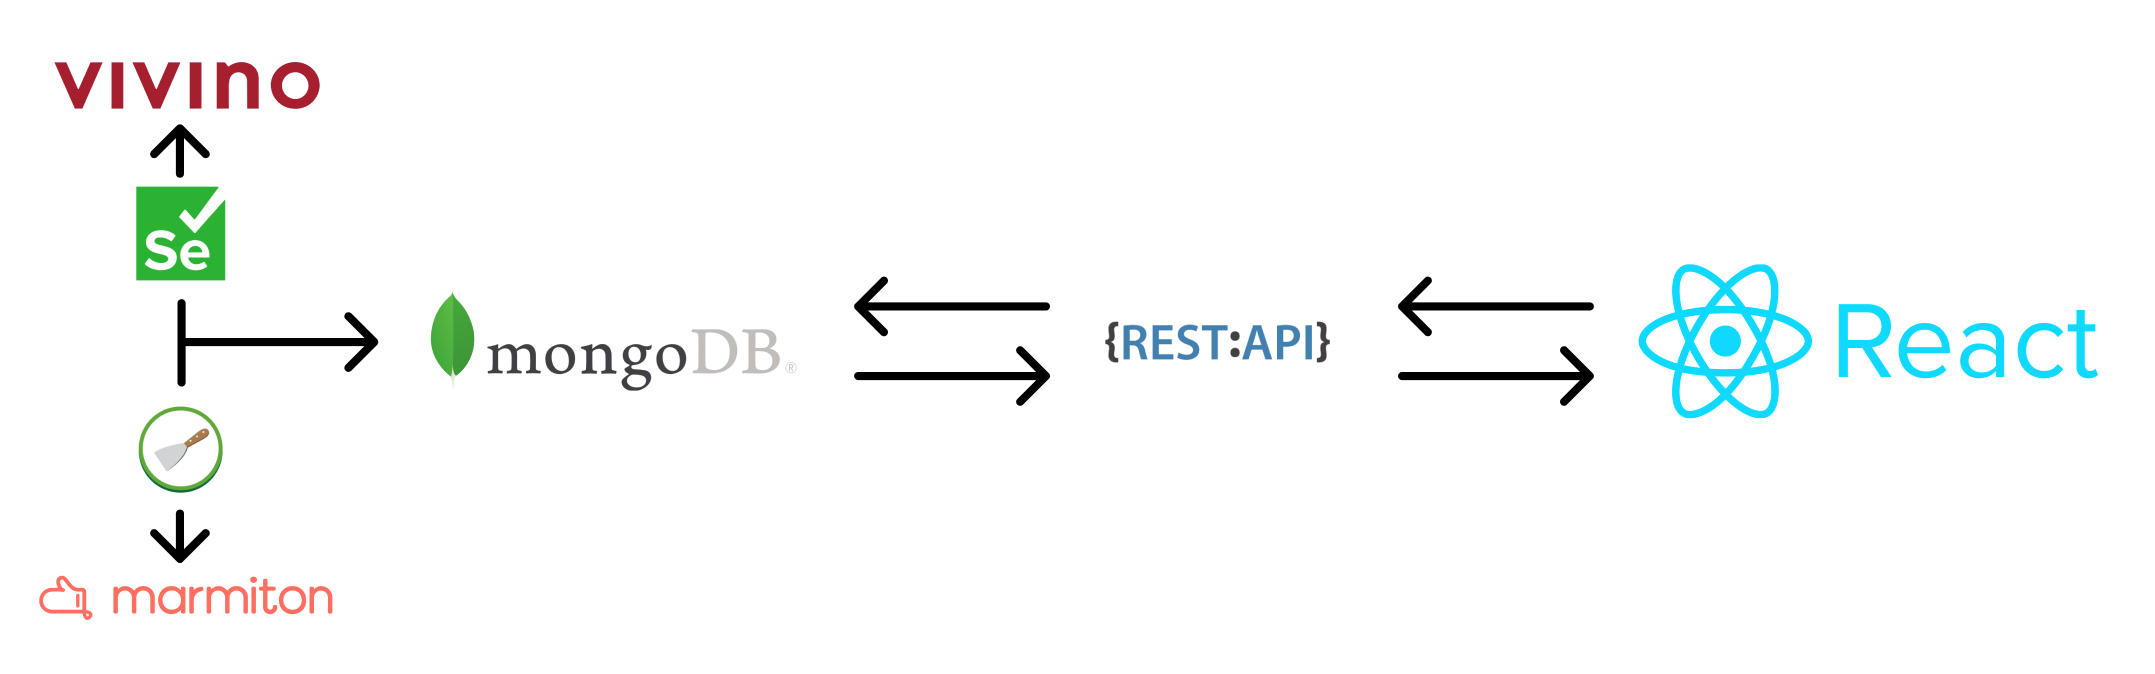
\includegraphics[width=0.8\textwidth]{rsc/architecture.png}
    \caption{Architecture globale du projet.}
    \label{fig:architecture}
\end{figure}


\section{Méthodes d'analyse}

Deux méthodes d'analyse sont envisagés dans ce projet. La première doit permettre recommander un vin pour une recette en comparant les listes d'accords des vins avec le nom et les ingrédients de la recette. La seconde doit permettre de déterminer si le vin est apprécié et les points qui le caractérisent en analysant les commentaires des utilisateurs sur les vins.

\subsection{Recommandation de vin}

Afin de recommander un vin suivant une recette, nous allons générer pour chaque recette une liste de vecteurs représentant son nom et ses ingrédients à l'aide d'un générateur d'embedding de mots comme Word2Vec ou GloVe. Pour chaque vin, nous procéderons de la même manière en générant une liste de vecteurs représentant les plats avec lesquels il s'accorde. La figure \ref{fig:word2vec} illustre la génération de ces vecteurs et leur stockage dans la base de données. Cette génération sera donc effectuée qu'une seule fois, sur toutes les données récupérées.

Ces vecteurs étant persistés dans la base, il sera possible de les récupérer une fois que l'utilisateur aura sélectionné une recette. Les similarités (par exemple la similarité cosinus) entre les vecteurs de la recette et ceux des vins seront ensuite calculées puis moyennées pour obtenir une note de recommandation. Une liste contenant les meilleurs vins s'accordant avec la recette sera alors retournée à l'utilisateur. La figure \ref{fig:recommandation} illustre ce processus.

% \begin{figure}[H]
%     \centering
%     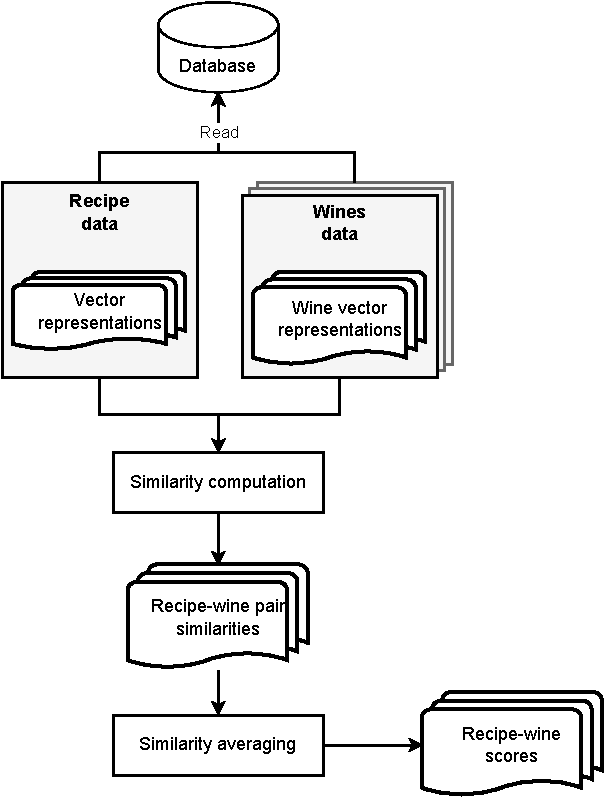
\includegraphics[width=0.4\textwidth]{rsc/similarities.pdf}
%     \caption{Processus de recommandation d'un vin pour une recette.}
%     \label{fig:recommandation}
% \end{figure}

\begin{figure}[H]
    \centering
    \begin{minipage}[b]{.5\textwidth}
      \centering
      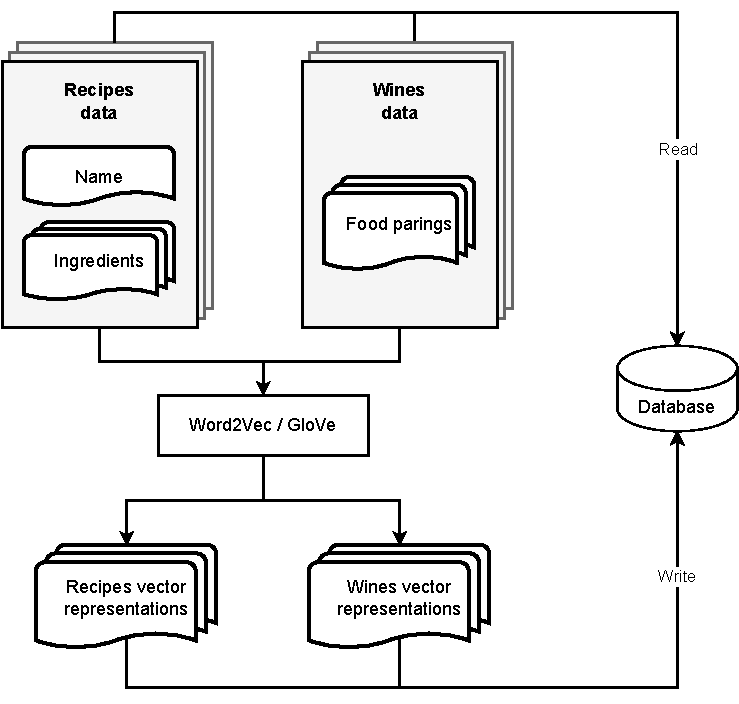
\includegraphics[width=.8\linewidth]{rsc/embedding_generation.pdf}
      \caption{\centering Processus de génération et de stockage des vecteurs représentatifs.}
      \label{fig:word2vec}
    \end{minipage}%
    \begin{minipage}[b]{.5\textwidth}
      \centering
      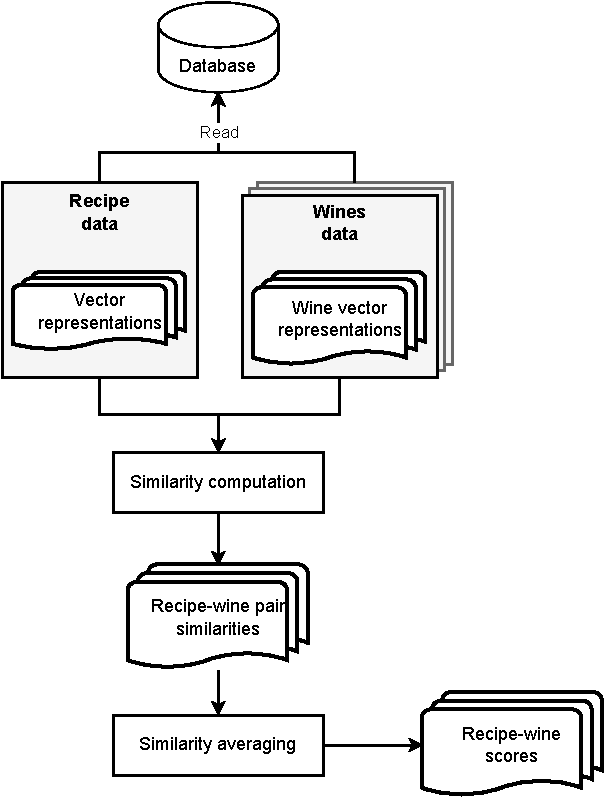
\includegraphics[width=.8\linewidth]{rsc/similarities.pdf}
      \caption{\centering Processus de recommandation d'un vin pour une recette.}
      \label{fig:recommandation}
    \end{minipage}
    \end{figure}

\subsection{Analyse des commentaires}
Afin d'analyser les commentaires, nous allons utiliser la librairie Python "pysentimiento". Cette librairie se base sur des modèles d'apprentissage profond Transformeur pour réaliser des tâches de traitement du langage naturel. Elle permet notamment de classifier un texte (dans notre cas le cas un commentaire) selon s'il est de nature positive, neutre ou négative, et également de générer le sentiment principal qui en ressort comme la joie, la tristesse ou encore la colère.

\vspace{10mm}
\newpage

%\uselandscape
  \chapter{Planning}
  La planification des tâches à effectuer pour la réalisation du projet est illustré par la figure \ref{fig:planning}. Chaque tâche est associée à un membre du groupe, représenté par une certaine couleur, à savoir:

\begin{itemize}
    \color{red}
    \item \textbf{Rouge}: \color{black}Andrea Petrucci
    \color{blue}
    \item  \textbf{Bleu}: \color{black}Benjamin Pasquier
    \color{orange}
    \item \textbf{Orange}: \color{black}Laurent Hirschi
    \color{teal}
    \item \textbf{Vert}: \color{black}Tout le monde
\end{itemize}

Les jalons sont de couleur 
\color{mygreen}verte \color{black} et les deliverables de couleur \color{red}rouge\color{black}.

\begin{figure}[H]
    \centering
    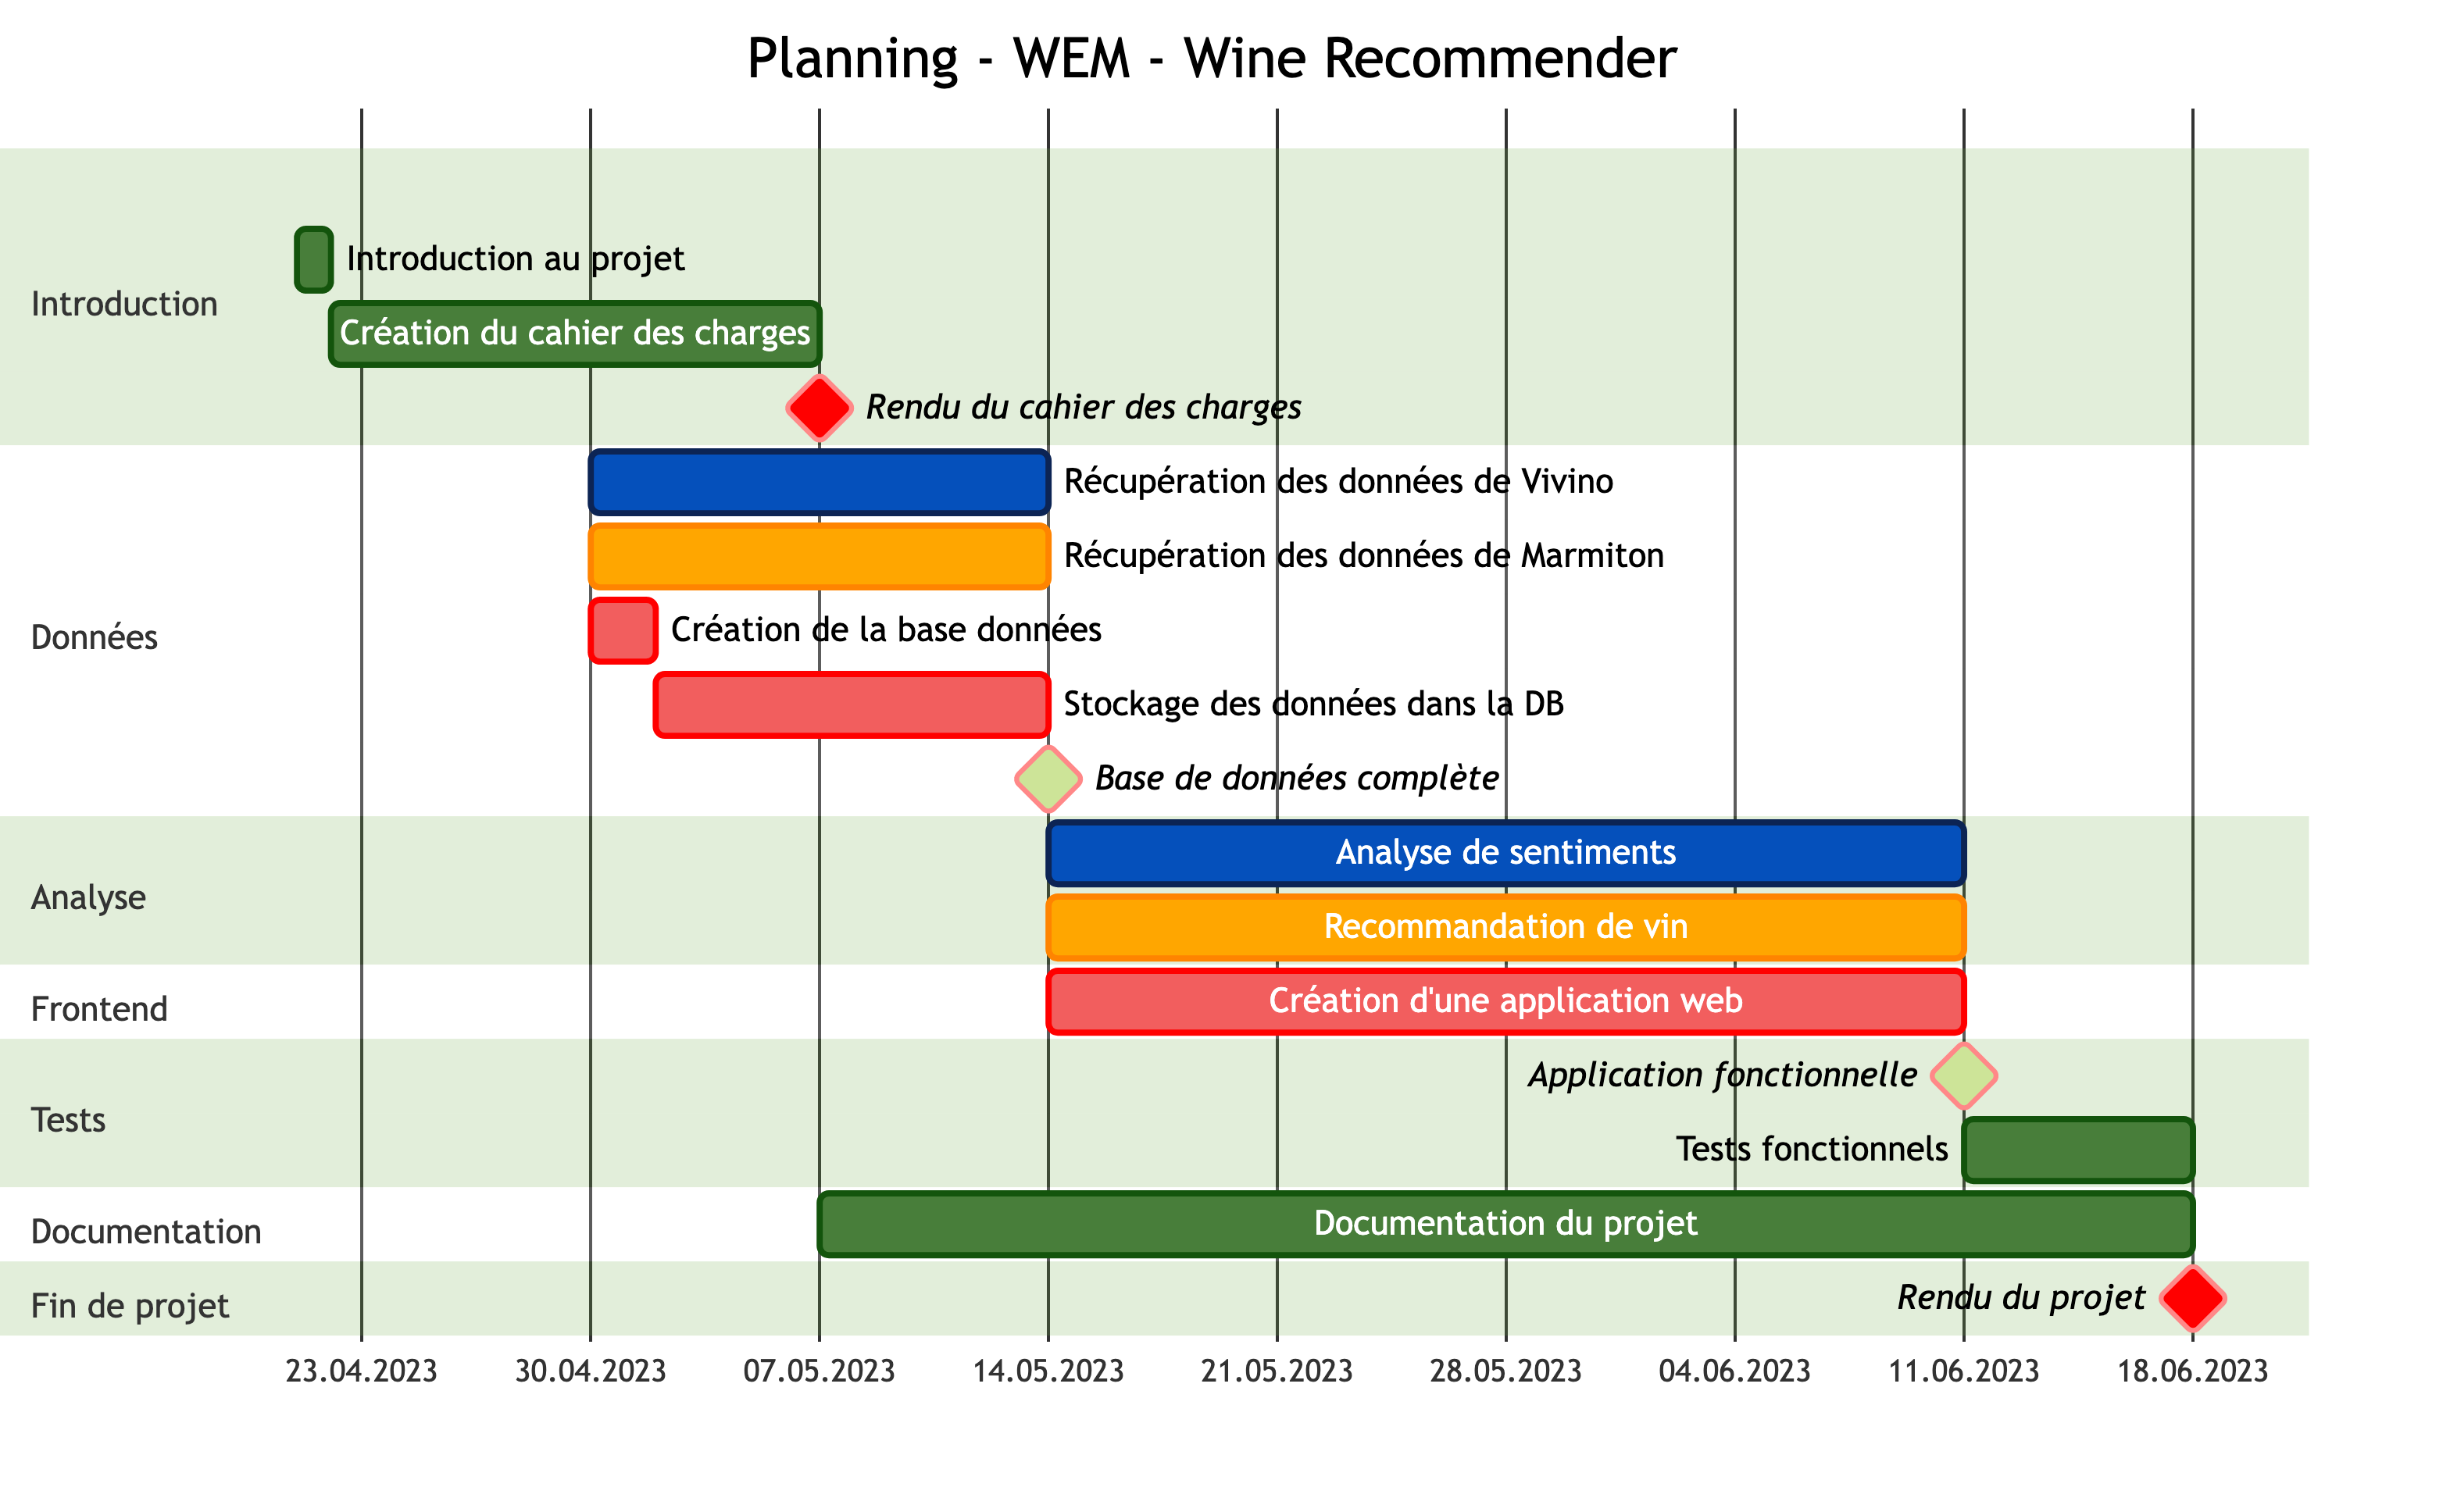
\includegraphics[width=1\textwidth]{rsc/planning.png}
    \caption{Planification}
    \label{fig:planning}
\end{figure}

%\useportrait
\newpage

\chapter{Résultats attendus et risques}
Ce dernier chapitre décrit les résultats attendus ainsi que les risques qui peuvent survenir lors de la réalisation de ce projet.

\section{Résultats attendus}

Le résultat final attendu est une page web qui permet à l'utilisateur de choisir une recette dans une liste ou en faisant une recherche. Une fois la recette choisie, l'utilisateur doit pouvoir voir les ingrédients nécessaires à la réalisation de la recette ainsi que les vins qui s'accordent avec cette dernière. Il doit également être possible de filtrer les recettes et les vins résultants en fonction de différents critères. Par exemple, on pourra filtrer les vins en fonction de leur prix, de leur pays d'origine, de leur type, etc. et les recettes en fonction des ingrédients nécessaires à leur préparation. La page web doit également retourner à l'utilisateur un sentiment décrivant les avis jugés utiles par Vivino. Ce sentiment doit être accompagné des mots les plus importants utilisés pour le jugement.

Bien entendu, il est attendu de l'application que les résultats retournés soient cohérents et que les vins proposés s'accordent bel et bien avec la recette choisie.

\section{Risques}

Quelques risques peuvent survenir lors de la réalisation de ce projet et ainsi influencer la qualité des résultats attendus.

\subsection{Précision de la recommandation}

Le premier risque est la précision de la correspondance des ingrédients. En effet, il est possible que la méthode de génération d'embedding et le calcul de similarité ne soit pas assez précis pour lier correctement les accords aux ingrédients de la recette. Dans ce cas, il sera nécessaire de trouver une autre méthode plus efficace. 

Il est également possible que les accords des vins soient souvent les mêmes et que l'application recommande souvent les mêmes vins pour des recettes différentes. Dans ce cas, il est difficile d'adapter la méthode puisque la cause du problème est le manque de diversité des accords des vins. Il serait donc nécessaire de trouver une autre source de données pour les accords des vins.

\subsection{Fiabilité de l'analyse des sentiments}

L'analyse des sentiments comporte également un risque. En effet, il est possible que les résultats de l'analyse ne soit pas fiable et que les avis jugés utiles par Vivino ne soient pas représentatifs de l'avis général des utilisateurs. Dans ce cas, il faudrait considérer une plus grande quantité d'avis utilisateur.

\subsection{Subjectivité du goût}

La subjectvité du goût est un risque sur lequel il est difficile d'agir, bien qu'il soit important de le mentionner. En effet, il est possible que les vins qui s'accordent avec une recette ne soient pas au goût de l'utilisateur. Il faudrait donc, si le temps le permet, ajouter une fonctionnalité permettant à l'utilisateur d'obtenir d'autres vins qui s'accordent avec la recette.
\newpage

%---Bibliography--------------------------------------------------------------%
%\bibliographystyle{ieeetr}
%\bibliography{bibliography/resources.bib}
%\addcontentsline{toc}{chapter}{Bibliographie}

\end{document}
